\chapter{A bibliographic database}
\label{ch:bibliography}

\section{Gathering publications in JabRef}
\label{sec:publicationsjabref}

Before you start searching for information, first prepare yourself to keep all sources in a structured way so that you can search for them later in a bibliograhic database. Bibliographies must be drawn up in a strict and documented manner. There are many different bibliography styles, but HOGENT has chosen one, the APA system (of the American Psychological Association)\footnote{\url{https://bib.hogent.be/how-to/bron-vermelden/ refereren -according to-apa6th/}}.

It is impossible to manually maintain a bibliography and entries in the text. Fortunately, there are several applications that specialized in maintaining a bibliographic database, so-called \emph{reference managers}.

HOGENT proposes Endnote, but Endnote is a commercial application, which you no longer have free access to after you graduate. This section introduces JabRef, an open source bibliographic record keeping application developed specifically for {\LaTeX}. JabRef uses the file format of Bib{\LaTeX}, the built-in bibliography system.

If you need more detailed information about Bib{\LaTeX} that is not in this guide, please refer to the manual~\autocite{LehmanEtAl2016}.

\begin{figure}
  \centering
  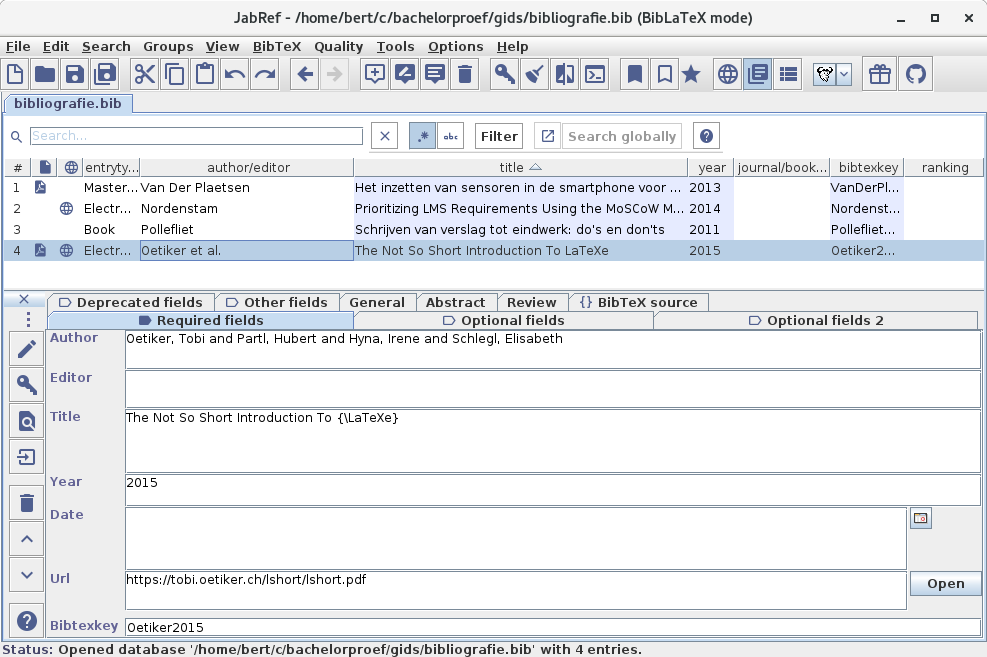
\includegraphics[width=\linewidth]{jabref-screenshot}
  \caption[JabRef]{\textbf{JabRef.} In the center of the user interface you will find an \emph{overview} of the different sources in this bibliographic database, in this case four. The \emph{pdf-icons} on the left of the first and fourth source indicate that the source is stored locally as a PDF. Clicking this will open the PDF. The \emph{globe icons} at the second and fourth source indicate a url that you can open in the web browser when you click on it. At the bottom is a \emph{detail pane} with the tracked data for the fourth source. These are divided into different tabs, including required data (``Required fields''), optional (``Optional'') and others (``Other fields''), etc. In this case, the names of the authors are filled in (see Section~\ref{sub:generalbibliographicaldata}). In this case there are no editors (``Editors''), and that field is left empty. The field ``Bibtexkey'' at the bottom is automatically generated (see Section~\ref{sub:jabrefsettings}) by clicking on the \emph{key symbol}.}
  \label{fig:jabref}
\end{figure}

\subsection{JabRef settings}
\label{sub:jabrefsettings}

You can download JabRef from \url{http://www.jabref.org/} and install it on Windows, MacOS and Linux. When you first open JabRef, it is useful to adjust the following settings:

\begin{itemize}
  \item In the menu, choose File > Switch to BibLaTeX mode. This makes the file format of the bibliographic database compatible with the {\LaTeX} template for the bachelor's thesis provided. To adjust this setting, you need to open a bib file.
  \item In the menu, choose Options > Preferences and then the category ``BibTeX key generator''. Each source in the database is identified by a unique key that you can have automatically generated. You can set its shape yourself. The default format is the first author's last name followed by the year of publication, eg ``Knuth1998''. You can adjust this to your own liking, but choose this beforehand and stick to it. You will use this key to refer to your sources from the text, eg with the command \verb|\parencite{Knuth1998}|.
  \item In the Preferences window, choose the File category and specify a directory for keeping PDFs of the sources found under ``Main file directory''. It is very interesting to download the articles found and keep them under that directory. Even better is to take the BibTeX key as the name of the file (eg Knuth1998.pdf). You can then easily open the file from JabRef.
\end{itemize}

You can check the other settings and adjust them to your liking, but the ones listed above are the most important.

\subsection{General bibliographic data}
\label{sub:generalbibliographicaldata}

The purpose of a bibliography is to allow the reader to look up your sources themselves and to assess them for reliability. This means that you must provide sufficient information so that the source can be found. Depending on the type of source (article in a journal, book, website, etc.) you have to provide different information. This will be explored further on. Three elements are \emph{always} essential: the \textbf{author}, the \textbf{title} of the source and the \textbf{year} (or date) of publication. If one of these three is missing, it becomes very difficult to evaluate the origin and quality of the resource. You can keep that kind of sources for information, but they are usually not suitable for inclusion in a bibliography. After all, if the author is unknown, it is not possible to judge whether he or she has the authority to write about the subject in an objective and in-depth manner. If the year is not specified, it is very difficult to determine to what extent this source has not yet been superseded by more recent developments in the field.

Some tips when entering author names:

\begin{itemize}

  \item Write the authors' names in the form ``Family Name, First Name(s)''. So ``Van Vreckem, Bert'' and not ``Bert Van Vreckem.'' In principle the second notation is also accepted, but this only works for typical Anglo-Saxon names with a middle name (eg ``Donald Ervin Knuth'' ). The first two words are considered as first names, the last word as the family name. In that case ``Van'' is therefore wrongly regarded as a middle name.
  \item If the author is a company or organization, with a name consisting of several words, enclose it in braces: eg ``\{The Linux Foundation\}''. If not, {\LaTeX} tries to interpret this as a person's name. ``Foundation'' then becomes the family name, ``The'' and ``Linux'' the two first names.
  \item If you have multiple authors, separate each name with \texttt{and}, eg ``Bernard, Anita and Buysse, Jens and Van Vreckem, Bert''.
  \item After entering the author name(s), click on the button with the key icon (see Figure~\ref{fig:jabref}) to generate a unique key for this resource.
  \item In addition to an author field, there is also a field for any editor(s) (\emph{editor}). At least one of the two must be completed, sometimes both. This happens, for example, in a book that is composed of chapters that are written by different authors and where you want to refer to one specific chapter. You will find an example of this further on in this text.
\end{itemize}

Note that in a bibliography, \textbf{only works referenced from the text} may be included. {\LaTeX} does this automatically by default, so if you're missing sources in the list, it means you didn't use them in the text.

Always try to keep as much information as possible about your sources, so that it will be easier to find them later. Although this is a time consuming process, and not all of this information is included in the bibliography, consulting the database is much easier. Pay sufficient attention to this and also check the result in the bibliography itself. Are the authors represented correctly? Do you have a year mentioned? Has a URL and date of consultation been specified for an online source (see below)? etc.

Some fields that are always useful to fill in:

\begin{description}
  \item[Abstract] Summary of the article. This is usually the first paragraph of an article and is always clearly marked.
  \item[DOI] or ``Digital Object Identifier''. This is a unique code for articles in scientific publications that makes searching easier (provided the DOI is given).
  \item[File] Name of the file containing the downloaded article. You can open the article from JabRef in a PDF viewer or text editor.
  \item[Keywords] Keywords representing the subject, separated by commas.
  \item[Review] Your own comments about this resource. Why did you keep this? What is the most interesting thing you learned from it?
  \item[URL] The URL where you found the article. This URL is not always included in the bibliography, but it is always useful to keep track of. You can open the website from JabRef in a web browser.
  \item[Urldate] the date on which you last consulted this source.
\end{description}

\subsection{Specific bibliographic data}
\label{sub:specific_bibliographic_data}

For the most relevant types of sources, this section explains how to properly track and include them in the bibliography. JabRef already gives some indications about which information is at least required: in the details window (see Image~\ref{fig:jabref}) you must at least fill in the tab ``Required fields''. For each type of publication below you will find an overview of the fields to be filled in, what they mean exactly, and what the reference in the bibliography will look like.

When adding a new source to a bibliographic database, you must first select the type (see Image~\ref{fig:jabref-entrytypes}). Below we only discuss the most important ones that are relevant for a bachelor's thesis.

\begin{figure}
  \centering
  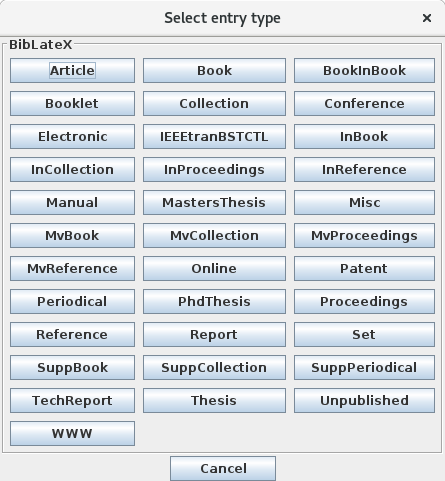
\includegraphics[width=0.6\linewidth]{img/jabref-entrytypes}
  \caption[Types of resources in JabRef]{\textbf{Types of resources in JabRef.} When adding a new resource in JabRef (Ctrl+N) you must first choose the type of publication. Depending on the type, different information must be provided in the bibliography.}
  \label{fig:jabref-entrytypes}
\end{figure}

\paragraph{Article}

This kind of source is only used for articles published in a scientific journal. Articles in magazines or newspapers are \emph{not} included. Required fields:

\begin{description}
  \item[Author] The name of the author;
  \item[Title] The title of the article;
  \item[Year] Year of publication;
  \item[Volume] The volume of the journal in which the article was published;
  \item[Number] The number (within the volume) in which the article appeared (sometimes not available);
  \item[Pages] Page numbers
\end{description}

Example:
\begin{verbatim}
@Article{SabiEtAl2016,
  author       = {Sabi, Humphrey M. and Uzoka, Faith-Michael E. and
                  Langmia, Kehbuma and Njeh, Felix M.},
  title        = {Conceptualizing a model for adoption of cloud
                  computing in education},
  journaltitle = {International Journal of Information Management},
  year         = {2016},
  volume       = {36},
  number       = {2},
  pages        = {183--191},
  doi          = {10.1016/j.ijinfomgt.2015.11.010},
  url          = {http://www.sciencedirect.com/[...]8401215001115},
  abstract     = {Cloud computing is a pervasive computing [...]},
  keywords     = {Cloud computing, Educational technologies, [...]},
  owner        = {bert},
  timestamp    = {2016-09-01},
}
\end{verbatim}

In the bibliography it looks like this: \fullcitebib{SabiEtAl2016}

\paragraph{InProceedings}

This kind of resource is used for articles published in the proceedings of a \emph{scientific} conference. Required fields:

\begin{description}
  \item[Author] Name of the author(s),
  \item[Title] Title of the article,
  \item[Booktitle] The name of the conference,
  \item[Year] The year in which the conference was held.
\end{description}

You can also optionally fill in the following fields:

\begin{description}
  \item[URL] to the conference website where the article can be found (possibly directly to the PDF);
  \item[Urldate] date on which you last consulted this source.
  \item[DOI] provided one is assigned to this item.
\end{description}

Example:
\begin{verbatim}
@InProceedings{VanVreckemEtAl2013,
  author    = {Van Vreckem, Bert and Borodin, Dmitriy and De Bruyn,
               Wim and Now\'{e}, Ann},
  title     = {A Reinforcement Learning Approach to Solving Hybrid
               Flexible Flowline Scheduling Problems},
  booktitle = {Multidisciplinary International Scheduling Conference
               (MISTA) 2013},
  year      = {2013},
  url       = {https://expertise.hogent.be/files/10711623/hffsp_la.pdf},
  urldate   = {2016-09-01},
  abstract  = {In this paper, we present a method based on Learning
               Automata to solve Hybrid Flexible Flowline Scheduling 
               Problems [...].},
  owner     = {bert},
  timestamp = {2016-09-01},
}
\end{verbatim}

In the bibliography it looks like this: \fullcitebib{VanVreckemEtAl2013}

\paragraph{InBook}

You use this type when you want to refer to a specific chapter in a book. At least the following fields must be completed:

\begin{description}
  \item[Author] The author(s) of the chapter,
  \item[Editor] The editor(s) of the book (if applicable),
  \item[Year] Year in which the book was published,
  \item[Title] Title of the \emph{chapter},
  \item[Pages] Start and end page of the chapter,
  \item[Booktitle] Title of the \emph{book},
  \item[Publisher] Name of the publisher.
\end{description}

Optionally, you can also add the following information:

\begin{description}
  \item[Subtitle or Booksubtitle] subtitle of the chapter or book, respectively,
  \item[Edition] Issue number,
  \item[Location] City where the publisher is located,
  \item[ISBN] The ISBN number of the book (for your information, never shown in the bibliography).
\end{description}

With a book it is unusual to provide a URL. If you want to keep track of the URL of the book on the publisher's website for your own information, it is best to do this in another field, e.g. Comment or Review.

Example
\begin{verbatim}
@InBook{Meyr2008,
  author       = {Meyr, Herbert},
  title        = {Forecast Methods},
  booktitle    = {Supply Chain Management and Advanced Planning},
  year         = {2008},
  editor       = {Stadtler, Hartmut and Kilger, Christoph},
  booksubtitle = {Concepts, Models, Software, and Case Studies},
  edition      = {4e editie},
  publisher    = {Springer},
  location     = {Heidelberg},
  isbn         = {978-3-540-24814-9},
  pages        = {461--472},
  comment      = {https://www.springer.com/us/book/9783540248149},
  owner        = {bert},
  timestamp    = {2016-09-02},
}
\end{verbatim}


In the bibliography it looks like this: \fullcitebib{Meyr2008}

%% TODO: boek, thesis, manual, \ldots

\paragraph{Electronic or Online}

This type of publication includes almost all online sources that cannot be classified under any other category: blog articles, articles in online professional journals or portal sites, YouTube videos of presentations at trade conferences, online documentation, etc.

Note that you may \emph{not} include the general website of organizations, software packages, etc. in your reference list. You should put this in a footnote.

The following fields are required:

\begin{description}
  \item[Author] Author(s) of the source, speaker (in case of a video of a lecture at a conference), \ldots
  \item[Title] Title of source, lecture, \ldots
  \item[Year] Year of publication (or possibly \textbf{Date}, the day of publication, if known),
  \item[URL] to the website where the source can be found,
  \item[Urldate] Date of last consult,
\end{description}

Many errors are made when referencing these types of sources. It is essential that the URL is provided and also the consultation date. The web is constantly changing, and it is possible that the content of a web page changes over time (e.g. bugs that are corrected) or even that a website restructures and thus the URL is no longer valid in some way. By specifying the date of consultation, you still offer the reader the opportunity to find out what that website looked like at that moment in time, for example via the Wayback Machine of the Internet Archive\footnote{\url{https://archive.org/web/}}.

Example of a blog article:

\begin{verbatim}
@Electronic{LewisFowler2014,
  author    = {Lewis, James and Fowler, Martin},
  title     = {Microservices: a definition of this new architectural
               term},
  date      = {2014-03-25},
  url       = {http://martinfowler.com/articles/microservices.html},
  urldate   = {2016-09-01},
  abstract  = {The term "Microservice Architecture" has [...]},
  keywords  = {application architecture, web services, microservices},
  owner     = {bert},
  timestamp = {2016-09-01},
}
\end{verbatim}

In the bibliography this becomes: \fullcitebib{LewisFowler2014}

Another example is one from a presentation at a trade conference that was published on Youtube. Because there is no separate field for mentioning the conference name, it has been incorporated in the title field.

\begin{verbatim}
@Online{Hykes2013,
  author       = {Solomon Hykes},
  title        = {The future of Linux Containers (PyCon 2013)},
  date         = {2013-03-21},
  url          = {https://www.youtube.com/watch?v=wW9CAH9nSLs},
  urldate      = {2016-09-01},
  abstract     = {At PyCon Solomon Hykes shows docker to the
                  public for the first time.},
  owner        = {bert},
  timestamp    = {2016-09-01},
}
\end{verbatim}

In the bibliography: \fullcitebib{Hykes2013}

\section{Searching for relevant information}
\label{sec:searchingforrelevantinformation}

The HOGENT library provides access to a large amount of scientific and professional literature that is not publicly available. This goes far beyond the books available in the library. After all, electronic sources (ebooks, magazines, etc.) can also be consulted. You can also find (good) bachelor's theses from previous years this way. The catalog can be consulted via \url{https://www.hogent.be/student/libraries/}.

\begin{itemize}
  \item Elsevier ScienceDirect
  \item Springer Online Journals
  \item Web of Science
  \item Google Scholar
\end{itemize}

Google Scholar is a search engine for scientific literature that searches both publicly available(``open access'') and paid publications. If you use Scholar from campus or via the VPN, you automatically have access to the publications to which the HOGENT library has a subscription.

Other publicly available search starting points:

\begin{itemize}
  \item Arxiv.org is a database of Open Access articles in a wide range of research domains, including the Computing Research Repository\footnote{\url{http://arxiv.org/corr/home}}.

  \item Wikipedia is a good starting point for your research, but remember that Wikipedia articles cannot serve as references themselves. So read the original sources of the article and use them if they are relevant to your bachelor's thesis.

  \item There are several portal sites for current ICT-related topics on which technical articles, presentations, interviews, etc. appear, e.g. dzone.com\footnote{\url{https://dzone.com/}}, infoq.com \footnote{\url{https://www.infoq.com/}}, etc.

  \item Search for conferences, workshops, symposia, etc. relevant to your field. You don't have to limit yourself to conferences in your own country! Examples are Devoxx\footnote{\url{https://devoxx.be/}} (Java), Google IO\footnote{\url{https://events.google.com/io2016/}} (Android), WWDC \footnote{\url{https://developer.apple.com/wwdc/}} (iOS), Configuration Management Camp\footnote{\url{http://cfgmgmtcamp.eu/}} (Linux Administrative Tools), etc.

        More and more conference lectures are filmed and published on Youtube or Vimeo \footnote{For Devoxx for example on \url{https://www.youtube.com/channel/UCCBVCTuk6uJrN3iFV\_3vurg}}. You can also look up the speakers and see if they have published their slides on Slideshare\footnote{\url{https://slideshare.net/}} or Speakerdeck\footnote{\url{https://speakerdeck.com/}} .

  \item Are there any local associations that are interested in your field? For example OWASP Belgium\footnote{\url{https://www.owasp.org/index.php/Belgium}} (security of mobile and web applications). You can search for such groups via Meetup\footnote{\url{https://meetup.com/}} or also via LinkedIn\footnote{\url{https://www.linkedin.com/}} (search specifically for groups such as the Belgian IT Infrastructure Network\footnote{\url{https://www.linkedin.com/groups/2092569}}). Check if there are any upcoming events near you and go there.

  \item Who are the most important names in the ``community''? Keynote speakers at conferences, authors of the most important books on the subject, etc. Follow these people on Twitter, find out if they have a blog, are active on LinkedIn, etc. Read all you can find they've written in the latest years.

  \item Find out if there are newsletters about your subject, which periodically send updates about current events in that field. Examples are Cron.Weekly\footnote{\url{https://www.cronweekly.com/}} (Linux System Administration), DevOps Weekly\footnote{\url{http://www.devopsweekly.com/}} or JS Weekly (and relatives)\footnote{\url{https://javascriptweekly.com/}}.
\end{itemize}

Keeping track of all your sources is time-consuming, but essential for a sound bachelor thesis! So pay the necessary attention to this and check whether the information about your sources is entered correctly in JabRef.

All relevant information that you have collected and read in the course of your research is then synthesized in a continuous text in your own words where you discuss the situation in the research domain, with references to the literature at appropriate places. We will go into more detail in Chapter~\ref{ch:reportingresults}.

\section{Summary}
\label{sec:bibliography-summary}

\begin{itemize}
  \item Set up your bibliographic database (e.g. with JabRef) before looking for information on your subject and store as much information as possible.
  \item Make sure you always write down at least the author, title and year of publication. Check for all other information required for this type of publication.
  \item In addition to consulting accessible sources, it is also interesting to find information about your subject via the HOGENT library.
  \item Use the APA style.
\end{itemize}
